\chapter{Circuits séquentiels}

\minitoc
%====================================================
\section{Introduction}
Nous sommes désormais armés pour représenter et manipuler les nombres sous forme binaire (chapitre 2), puis les traiter par une électronique numérique (chapitre précédent).
Toutefois, les opérateurs étudiés jusqu'ici se bornaient à des traitements combinatoires. En aucune manière, nous ne nous sommes autorisés jusqu'ici à prendre
en compte des valeurs du passé. En particulier, {\bf il nous est interdit de reboucler un signal sur le nuage combinatoire dont il est issu}.
Par exemple, il nous est jusqu'ici impossible de réaliser directement un circuit qui réalise une suite numérique comme : $$u_{n}=u_{n-1}+42,n \in  \mathbb{N}^+$$

Les circuits que nous allons considérer désormais sont appelés circuits {\it séquentiels}.
Nous nous intéressons ici, précisément à l'indice des suites précédentes : on considère que les indices successifs représentent des instants logiques discrets.
Pour parler de la valeur précédente du signal $u_n$, nous devons nous doter d'un moyen électronique de franchir un nombre de "pas temporels".
Par la suite, nous parlerons de "cycles" (ou "coup d'horloge") plutôt que de "pas temporels".
Ainsi, dans la suite précédente, il existe un cycle entre entre $u_n$ et $u_{n-1}$. C'est donc une seconde discrétisation --celle du temps-- qui nous préoccupe ici, après celle qui consistait à discrétiser les valeurs d'un signal.
Ces circuits, qui sont à même de se référer à des valeurs du passé, sont des circuits {\it séquentiels}.

\section{Discrétiser le temps}

\paragraph{Eviter la "cacophonie"}

Les circuits combinatoires précédents se présentent sous la forme d'un nuage : ses comportements sont, d'un point de vue microscopique, très complexes à analyser. Ainsi, si l'on
disposait d'un oscilloscope suffisamment précis, on constaterait un très grand nombre d'événements (ou "oscillations" ou "changement de valeurs") {\it internes} fluctuants dans le temps et donc d'une mesure à l'autre.
\begin{center}
  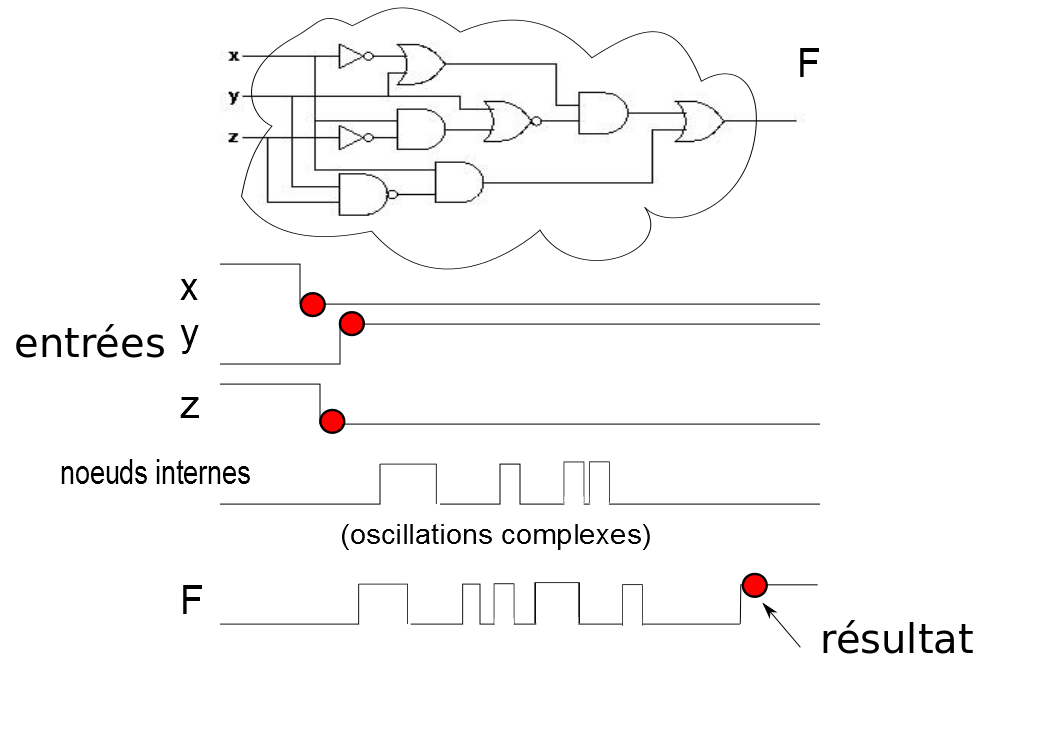
\includegraphics[width=12cm]{./figures/cloud-complexe-events.png}
\end{center}


De même, aux bords du circuit, sur les entrées-sorties, ces événements apparaissent au gré des stimulations extérieures (générateurs de signaux, capteurs, etc), parfaitement {\it asynchrones} : par ce terme
"asynchrone", on indique qu'il n'existe pas a priori de référentiel temporel qui puisse donner un "tempo" commun à tous.
Nous cherchons donc ici à trouver un moyen d'éviter cette cacophonie qui semble se profiler, et toutes les tracasseries d'ingénieurs qui lui
seraient liées. On observe d'ores-et-déjà qu'il semble suffire d'attendre un temps "suffisamment long" pour que le signaux se stabilisent et que les
sorties délivrent leur résultat attendu. Une fois que l'on est sûr que ce temps long est respecté, l'ordre interne qui a mené au résultat final n'importe plus.

\paragraph{Notion d'horloge périodique}
Le moyen technique de créer de l'ordre dans la succession des évènements d'un circuit est de recourir à une horloge commune.
Cette horloge est ici un signal carré, parfaitement périodique, de période $T$. Là encore, l'analogie musicale s'impose : à la manière d'un chef d'orchestre, l'horloge vise à donner un rythme unique et commun à tous les éléments en présence.
Il serait  possible de préciser le ratio entre le temps du signal à '1' et à '0', mais comme nous allons le voir ceci n'est pas d'un grand intérêt : en effet, au sein de ce signal carré, nous allons
uniquement nous intéresser au {\it front montant} de cette horloge. Idéalement, ce front montant peut être vu comme instantané. Par analogie avec les mathématiques du traitement du signal,
l'ensemble des fronts montants peut être vu comme un {\it peigne de Dirac} parfait, ou "shah" de Dirac \footnote{Toutefois, même si cette référence mathématique
est intéressante, elle a ses limites et n'est guère référencée par les Electroniciens. La raison en est simple : en général les traiteurs de signaux font une hypothèse algorithmique
forte qui consiste à supposer que le signal est {\it disponible}, dans son intégralité, au moment du calcul. L'Electronicien quant à lui s'inquiète plus de la manière de capter et traiter ce flux, souvent à la volée ({\it streaming})}.
\begin{center}
   \begin{minipage}[t]{4cm}
     \vspace{0pt}
     \centering
     $$\Sh(t)=\sum_{n=-\infty}^{n=+\infty}\delta(t-nT_e)$$
   \end{minipage}%
   \begin{minipage}[t]{8cm}
     \vspace{20pt}
     \centering
     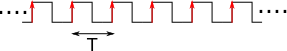
\includegraphics[width=6cm]{./figures/shah_dirac.png}
   \end{minipage}
\end{center} % added ending }

\section{Bascule D}
La bascule D est l'élément clé de notre discrétisation du temps. C'est le seul élément électronique sensible au front montant de l'horloge. La bascule D n'est donc pas une "nouvelle porte logique",
mais a un status particulier et un fonctionnement particulier. Néanmoins, il est d'usage de présenter sa table de vérité, en analogie avec les portes logiques. Alors que les entrées
d'une table de vérité classique font apparaître des valeurs logiques, ici la table fait intervenir le front montant.\\
\begin{center}
   \begin{minipage}[t]{8cm}
     \vspace{0pt}
     \centering
     \includegraphics[width=8cm]{./figures/d-ff-infos.jpg}
   \end{minipage}
\end{center} % added ending }
La fonction basique de cette bascule D est de réaliser une copie de son entrée 'D' sur sa sortie 'Q'. Cette copie a lieu sur le front montant de l'horloge. Il faut physiquement
un très court temps de propagation entre le signal d'horloge et la sortie, appelé "clock-to-Q". Ce temps physique est à prendre en compte à un moment ou un autre,
mais n'oublions pas notre but initial de nous "dépolluer" de toute préoccupation d'ordre "physique", pour nous concentrer sur la réalisation mathématique de notre suite numérique (discrète).
La fonction de copie semble donc bien modeste. Elle assure pourtant la distinction entre une valeur "avant" et une valeur "après" le front montant d'horloge. En dehors
de ce bref instant d'échantillonnage, la bascule D conserve la valeur précédemment échantillonnée.

\subsection{Fonction d'échantillonnage de la bascule D. Set-up et hold. Metastabilité.}
Une première utilisation intéressante de la bascule D est qu'elle permet d'échantillonner un signal d'entrée qui varie de manière plus rapide que l'horloge.
Pour que cet échantillonnage se passe correctement, la bascule doit être utilisée dans des conditions particulières : notamment, il est nécessaire que le signal (numérique)
à échantillonner soit {\it stable} un peu avant et un peu après le front montant. Ces deux temps à respecter s'appelle respectivement le temps de {\it set-up} et de {\it hold}.
Si par mégarde ou malchance, le signal d'entrée fluctue précisément à cet instant, la bascule entre dans un état particulier dit {\it métastable}. Cet état ne permet
pas de garantir avec certitude que le bon '0' ou le bon '1' apparaîtront en sortie de la bascule. Pire, cette sortie peut même se mettre à fluctuer sans sembler pouvoir
se stabiliser.

\begin{center}
  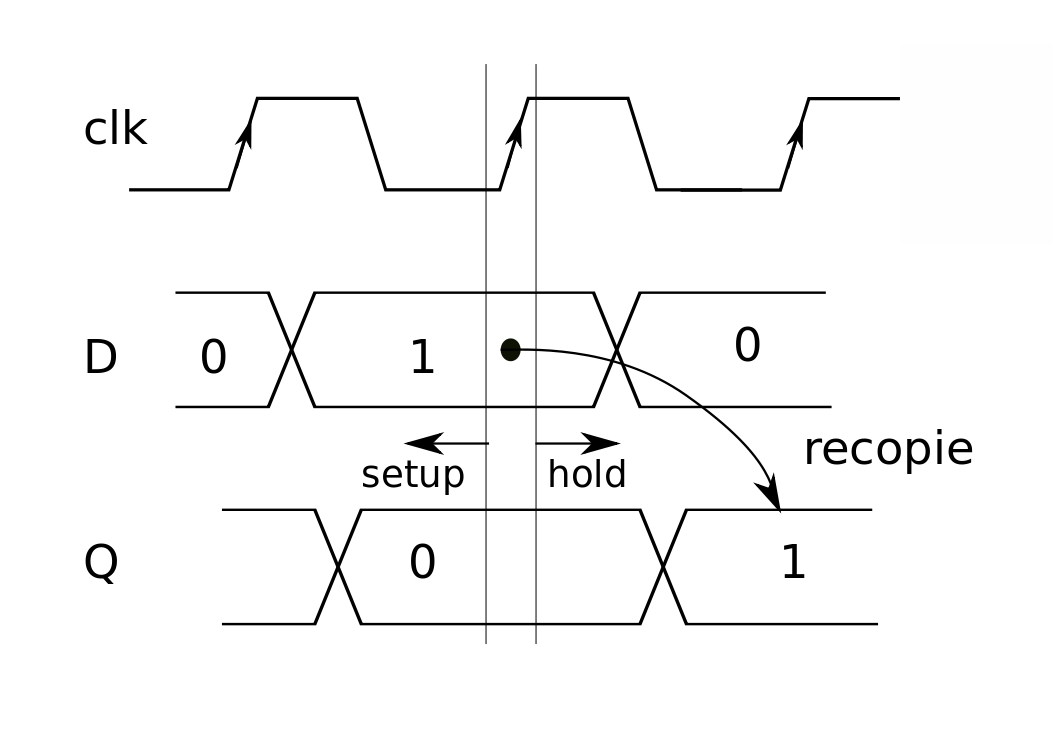
\includegraphics[width=6cm]{./figures/dff-chrono.png}
\end{center}

\subsection{Décalage temporel : la raison d'être de la bascule D}
La véritable raison d'être de la bascule est qu'elle permet de décaler un signal d'entrée d'un cycle d'horloge : le signal Q ne pourra en effet être "vu" d'un calcul en aval qu'au
cycle d'horloge qui suit.

\begin{center}
  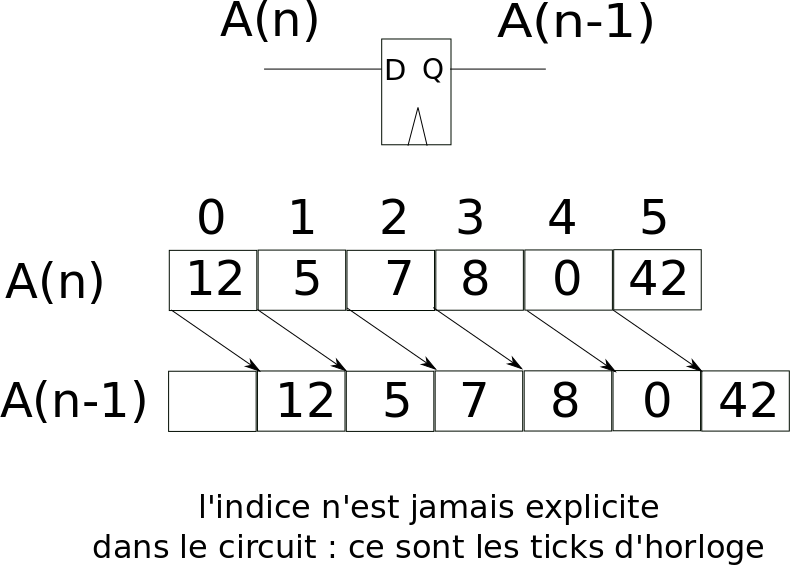
\includegraphics[width=9cm]{./figures/DFF_decalage_temporel_timed.png}
\end{center}

\section{Quelques {\it patterns} de conception synchrone}

Tout système numérique, simple ou complexe, est une combinaison de portes logiques et de bascules D.
Un tel assemblage générique est présenté sur la figure suivante : on observe un enchaînement de traitements
combinatoires et de bascule D. Des rebouclages peuvent exister, mais il doit forcément exister une bascule D sur les chemins
concernés : aucune chemin bouclé sur lui même ne peut être purement combinatoire. Ce schéma générique peut être décliné dans une
très grande variétés de patterns de conception. Le pattern le plus étudié est probablement les automates d'états finis ("FSM" : finite state machine), auquels
nous consacrons le chapitre suivant.

\begin{center}
  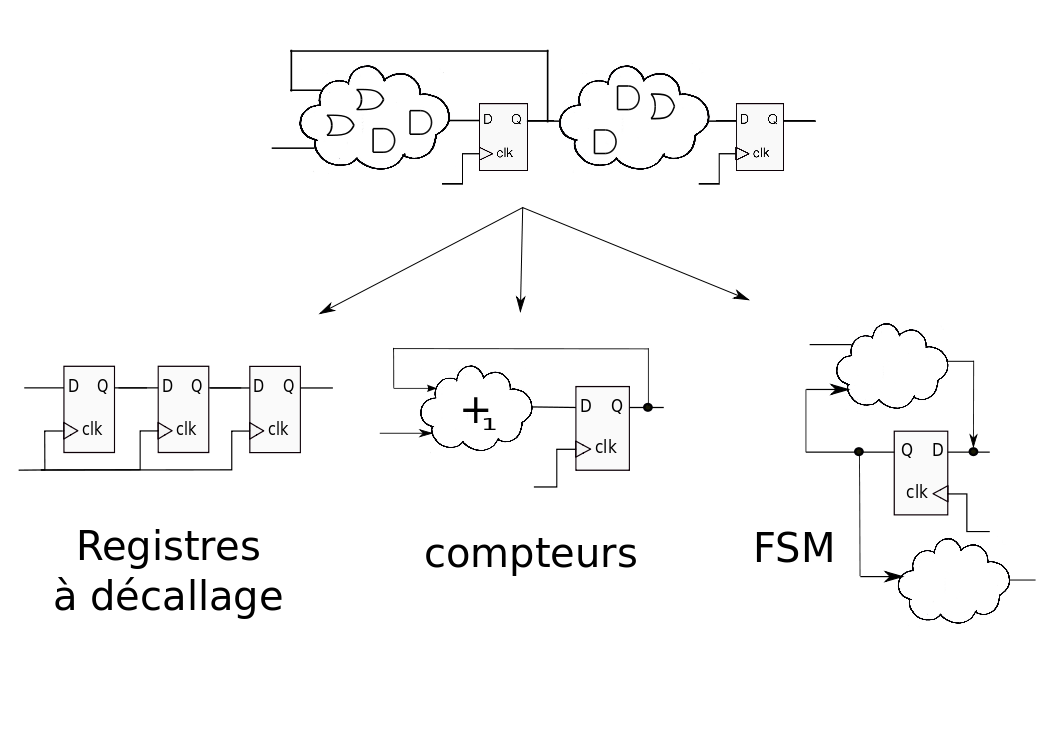
\includegraphics[width=10cm]{./figures/synchrone.png}
\end{center}

Pour l'heure, on peut citer quelques autres circuits numériques connus, qui font usage de la bascule D \footnote{En Informatique théorique , l'importance des automates est telle
que ces circuits électroniques sont vus comme de automates particuliers. L'Electronicien ne fera pas cet amalgamme.}.

\subsection{Registre à décalage}
Les registres à décalage sont des assemblages linéaire de bascule D, chaînées les unes à la suite des autres. Lorsqu'une donnée se présente, la précédente est déjà
dans le premier étage, et l'avant-dernière dans le deuxième étage etc. A chaque front montant d'horloge, de manière synchrone, toutes les bascules prennent leur entrée et modifient
leur sortie Q, {\it en même temps}. C'est une forme primitive de traitement parallèle. A titre de curiosité, la simulation logicielle d'un tel dispositif n'est pas immédiate ; il faut doubler
le nombre de variables et calculer dans un premier temps les {\it états futurs} de toutes les bascules, puis, dans un second temps,  réaliser la mise à jour de toutes les variables.
Le décalage synchronisé de ces registres est fascinant et confine à l'harmonie. Toutefois, on ne peut manquer de faire la comparaison avec le travail à la chaîne : le taylorisme, né
dans l'industrie de l'automobile s'en est grandement inspiré (voir "les temps modernes" de Charlie Chaplin) !


\begin{center}
  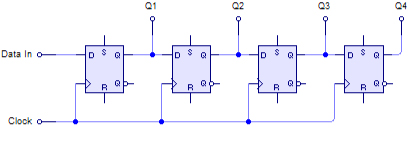
\includegraphics[width=6cm]{./figures/Shift_Register.png}
\end{center}

\subsection{LFSR : linear feedback shift register}
Les LFSR ont l'intérêt de créer de manière simple des suites en apparence aléatoires. En réalité, les suites
de valeurs produites sont pseudo-aléatoires et parfaitement récurrentes à partir d'un certain rang. La simplicité
des LFSR les rendent malgré tout très attrayants dans de nombreuses situations. Noter la présence d'un ou plusieurs OU exclusifs, qui
sont les véritables "créateurs de désordre" au sein de la suite. La place de ces Xor peut être définie à l'aide de polynômes générateurs.
\begin{center}
  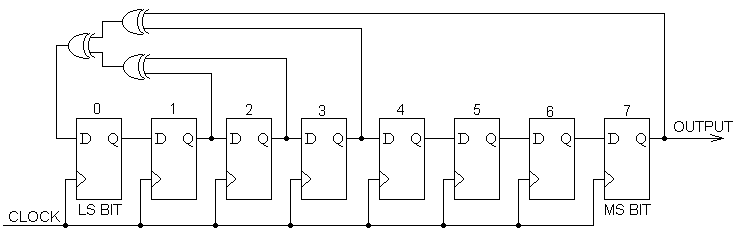
\includegraphics[width=9cm]{./figures/lfsr.png}
\end{center}

\subsection{Bascule D et multiplexeur : mémorisation}
La seule fonction de décalage semble très éloignée des fonctions que l'on peut attendre d'un processeur numérique. De fait,
la bascule D est le plus souvent utilisée conjointement à un multiplexeur. Ce multiplexeur (combinatoire) permet de sélectionner
à volonté l'action d'{\it échantillonner ou non} : le signal de contrôle du multiplexeur permet effectivement soit de router le signal vers l'entrée D de la bascule, soit
de refaire circuler la donnée précédemment stockée dans la bascule, au coup d'horloge précédent. On parle effectivement de {\it recirculation} de la donnée Q, qui tourne
en boucle de la sortie, vers l'entrée etc : la donnée est ainsi piégée. Ce piégeage est une {\it mémorisation}. Très souvent, ce mécanisme est présenté comme
intégré au sein de certaines bascules, tant il est commun : le signal de contrôle du multiplexeur s'appelle alors un {\it enable}. Lorsque l'enable est à '1',
la donnée présentée en entrée est effectivement échantillonnée, sinon, c'est la valeur précédente qui reste "occupe" la bascule.

\begin{center}
  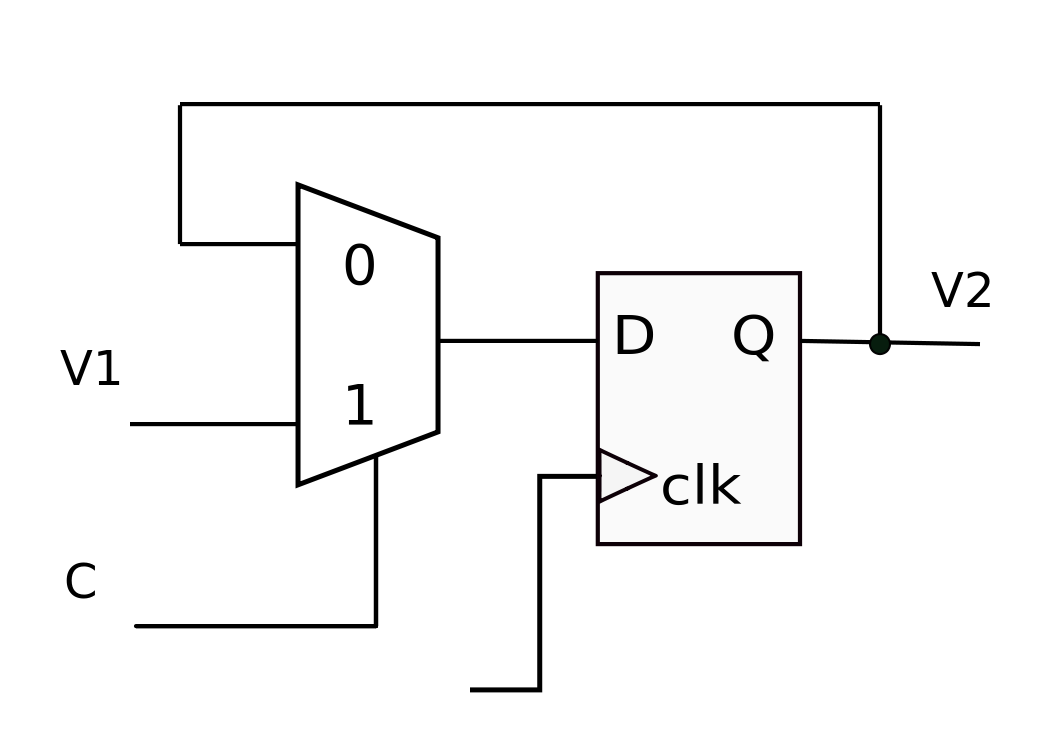
\includegraphics[width=5cm]{./figures/dff-enable.png}
\end{center}


\subsection{Compteurs et timers}
La fonction d'un compteur est d'incrémenter un registre. Cet incrément peut se faire sur tous les 'top' d'horloge, ou de manière commandée en utilisant un signal d'autorisation.
Les compteurs peuvent notamment servir à réaliser des {\it timers} : ces dispositifs très importants en embarqué permettent d'interrompre un circuit au bout d'un certain temps. Ce temps
correspond à la valeur limite d'un compteur. L'intérêt de ces timers est par exemple de laisser un processeur réaliser une fonction principale, et de le détourner périodiquement vers une tâche annexe : c'est la notion
d'{\it interruptions}.

\begin{center}
   \begin{minipage}[t]{8cm}
     \vspace{0pt}
     \centering
     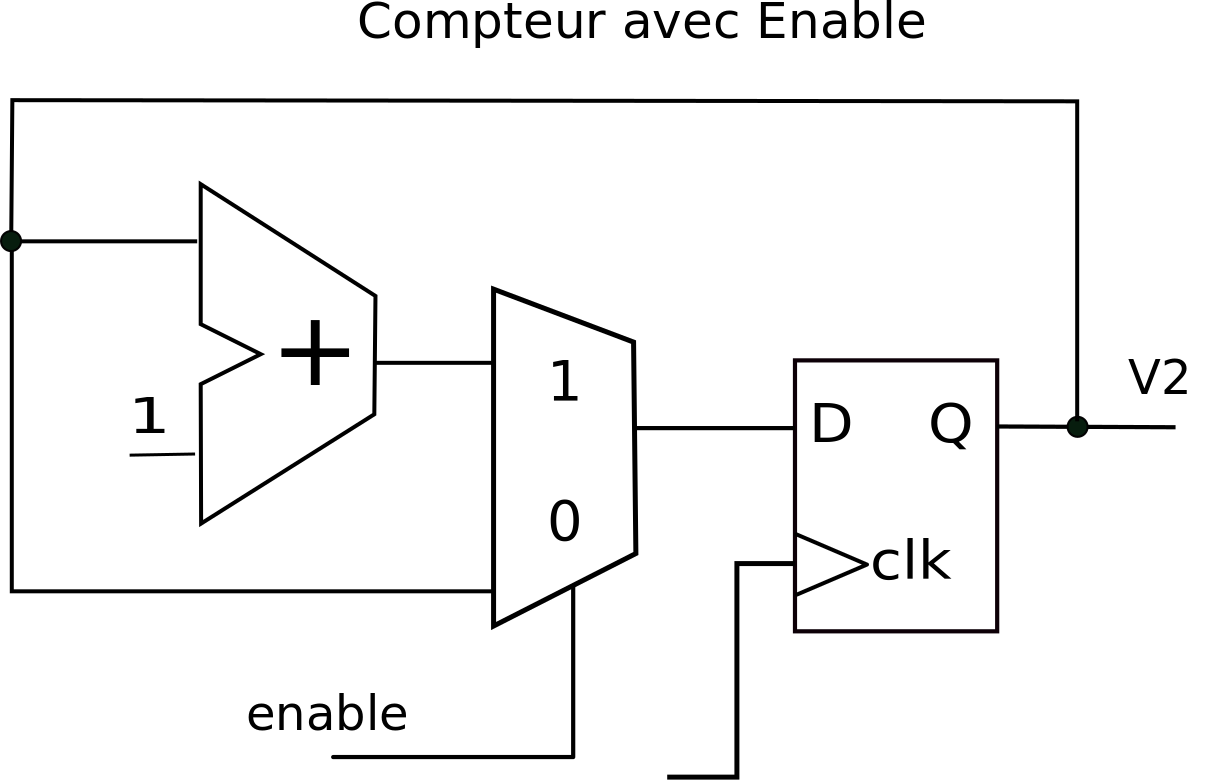
\includegraphics[width=6cm]{./figures/compteurs.png}
   \end{minipage}

   \begin{minipage}[t]{8cm}
     \vspace{0pt}
     \centering
     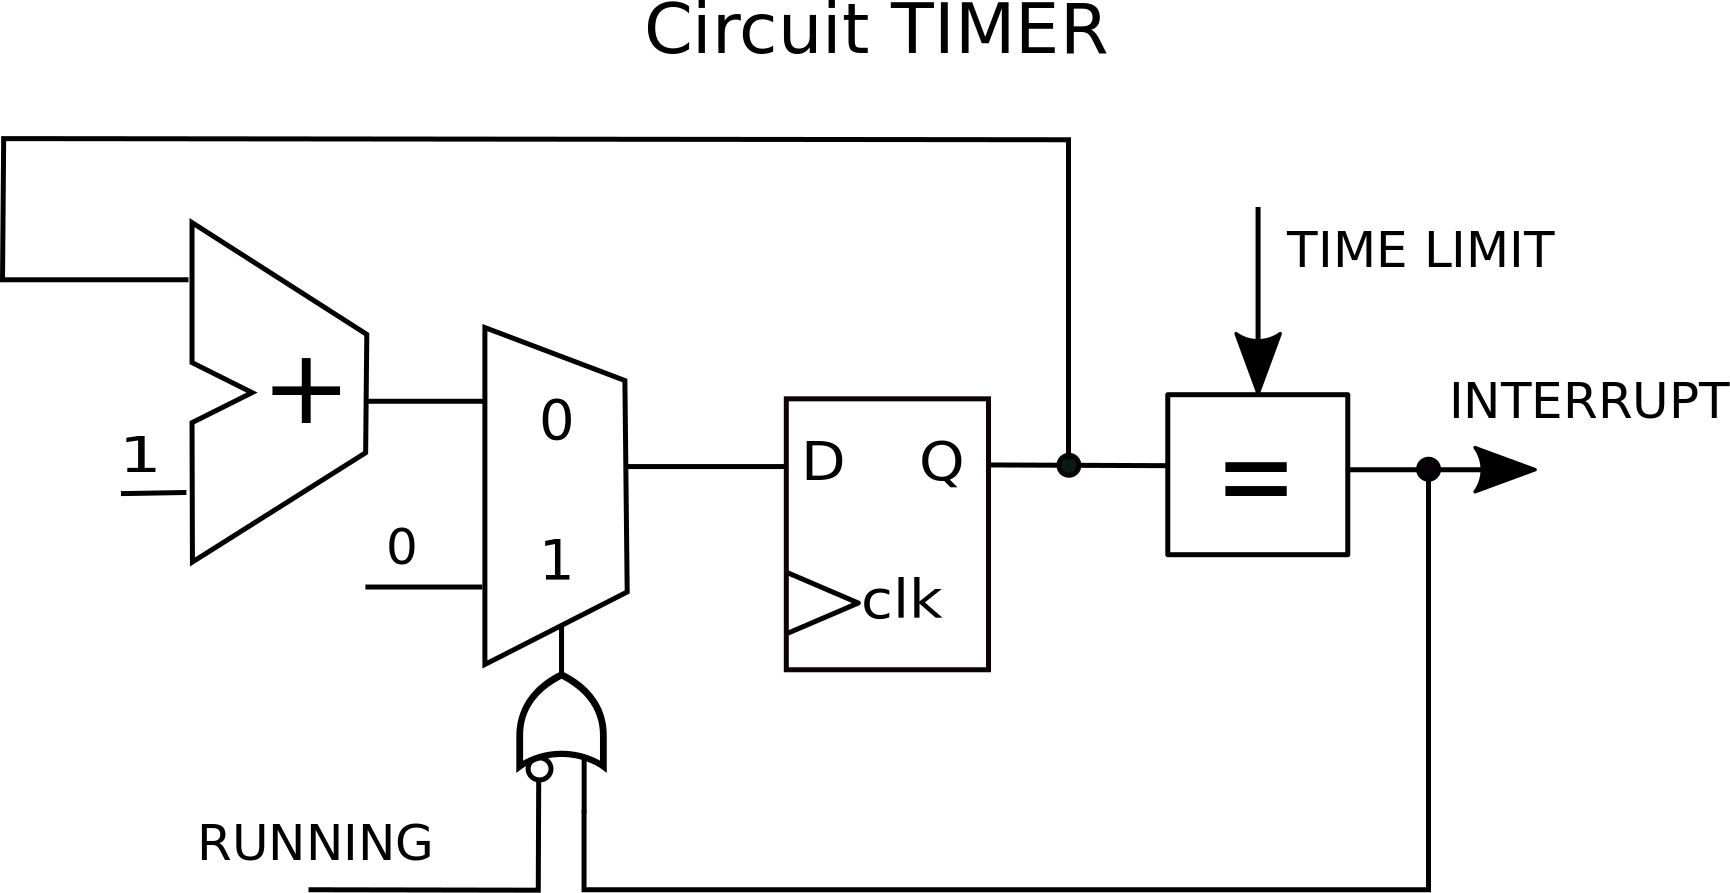
\includegraphics[width=6cm]{./figures/timer.png}
   \end{minipage}

\end{center} % added ending }


%====================================================
\section{Initialisation d'une bascule D}
Les symboles précédents des bascules D sont incomplets ; deux signaux importants n'y figurent pas, à savoir : le signal "set" et le signal "reset".
Ces signaux interviennent au tout démarrage du circuit, à sa mise sous tension : ce temps particulier s'appelle la phase de {\it reset du circuit}.
A cet instant particulier (qui dure quelques millisecondes), il est nécessaire de placer toutes les bascules D dans un état connu ('0' ou '1'), bien maîtrisé.
Cette mise sous tension provient d'une action extérieure (appui sur le bouton de la télé, etc), qui prendra fin pour laisser place au régime permanent.
Le signal "set" sert à initialiser la sortie Q de la bascule à '1', tandis que le signal "reset" place cette sortie Q à '0'. Cette prise en compte
est {\it asynchrone} : les signaux "set" et "reset" sont prioritaires sur l'horloge. Après la phase de reset, c'est le régime permanent qui s'établit :
l'horloge reprend alors "tous ses droits" et est la seule à commander la valeur de la sortie Q (recopie de D). Ce régime permanent est généralement
considérablement plus long que le régime transitoire de reset. Si, pour une raison ou une autre, les signaux de set ou reset sont à nouveau
utilisé, ils reprendront instantanément la "main" sur la sortie Q, et imposeront une nouvelle sortie Q. Mais encore une fois, le schéma classique
de fonctionnement est : phase de reset suivi d'un très long régime permanent.

\begin{center}
  \includegraphics[width=7cm]{./figures/d-ff-full.jpg}
\end{center}

Pour bien mettre en oeuvre la phase de reset, on peut observer les équations d'implication suivantes, qui résument le mécanisme d'initialisation :
\begin{itemize}
  \item $set=POL_s \implies Q=1$
  \item $reset=POL_r \implies Q=0$
\end{itemize}
Elles font intervenir un couple ($POL_s,POL_r$). POL dénote la {\it polarité} sur set ou du reset, placé en indice. La polarité indique quelle est la valeur
logique active : par exemple si $POL_s=0$, cela signifie qu'il faudra produire un $0$ sur le signal set pendant le démarrage, pour que que l'on obtienne
l'effet escompté sur $Q$, à savoir $Q=1$. Notons que sauf exception, on a $POL_s=POL_r$.
La polarité est également signalée sur les schémas par un petit cercle (présent ou absent) près du signal set ou reste de la bascule : la présence du cercle
indique une polarité à '0' et '1' en cas d'absence.
Lors du régime permanent, il faudra s'assurer que les signaux set et reset n'ont aucune influence sur $Q$ et donc
qu'ils sont bien commandés. S'ils sont commandés avec une valeur différente de leur polarité, ils n'auront aucun effet. Lors de la conception, il
faut donc s'assurer que l'on relie correctement les boutons de reset à ces signaux, avec les bonnes polarités : par exemple, il faudra se poser la question
concernant l'appui sur le bouton : cet événement produit-il une tension à '0' ou à '1' ? Et quelle est la polarité des signaux de reset de la bascule ?

\paragraph{Exemples}
Nous donnons ici deux exemples (voir schémas) impliquant 2 bascules D et un signal de reset arrivant de l'extérieur. Supposons que l'on cherche à initialiser les bascules dans l'état $Q_1=0$ et $Q_0=1$.
On suppose que le signal de reset est actif haut : lorsqu'on appui sur le bouton de reset, le signal devient '1'. Lorsqu'on le relache, il repasse à '0'. Pour initialiser les bascules,
 il faut jouer sur les signaux set et reset des 2 bascules : cela fait 4 signaux à connecter de manière appropriée. Aucun signal ne doit rester non connecté (aucun signal "en l'air").
 \begin{itemize}
   \item Dans le cas du schéma de gauche, la solution consiste d'une part à connecter le signal reset à l'entrée reset de la bascule $Q_1$ et au set de la bascule $Q_0$. Les autres entrées des bascules doivent être connectées, même si elles sont inactives : il suffit
   de les connecter à la masse (0).
   \item Dans le cas du schéma de droite, il faut adapter la polarité du signal de reset (actif haut) pour activer correctement le reset de la bascule (présence d'un cercle $\implies$ polarité à 0).etc
 \end{itemize}


 \begin{center}
   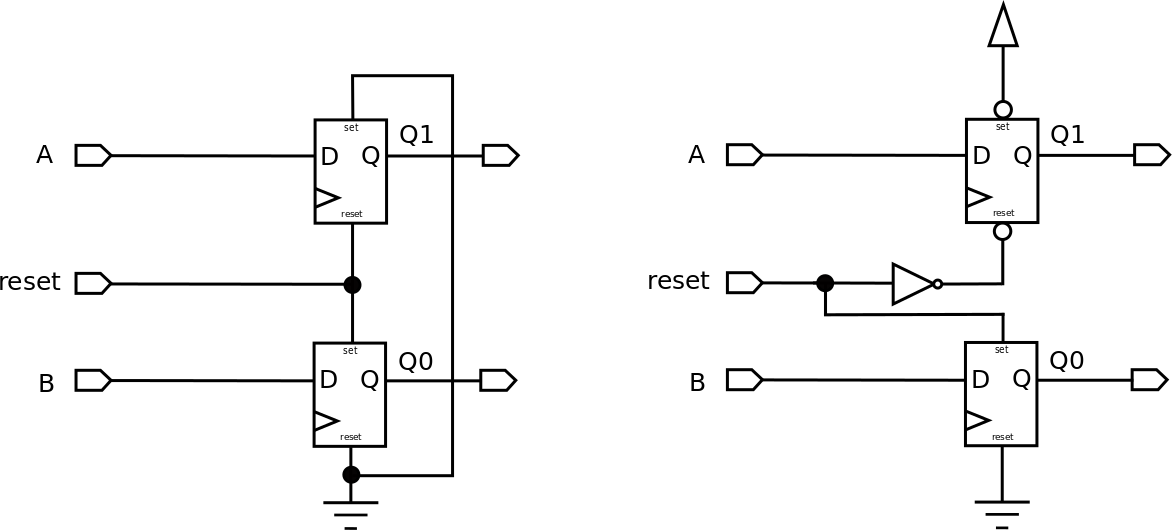
\includegraphics[width=8cm]{./figures/dff_init.png}
 \end{center}

\paragraph{Simplification grâce aux HDL}
Le mécanisme de reset peut être perçu comme relativement complexe. Qu'on se rassure : les langages de descriptions matérielle, dont VHDL (étudié plus loin),
masque totalement ce travail de fourmi consistant à réaliser ces câblages minutieux.

%=====================================================
\section{Conclusion}
Ce chapitre nous a permis de nous doter de l'élément clef des systèmes séquentiels, à savoir la bascule D. Nous avons pris le parti de ne pas "ouvrir le capot" de la bascule D, alors
que c'est souvent ce que s'empresse de faire de nombreux manuels. Les raisons en sont multiples : d'une part les HDL reposent uniquement sur la synthèse de bascules D ; d'autre part, sous le capot
de ces bascules, plusieurs types de structures peuvent apparaître, la plus connue étant la bascule RS asynchrone. C'est un montage tête-bêche de 2 portes logiques NOR (ou NAND) : la sortie de l'une est câblée sur l'autre et l'ensemble
présente un cycle combinatoire que nous avons tenté de totalement exclure (règle de base : pas de boucles combinatoire en conception numérique !). A notre sens, ces deux seules raisons, associées à un temps d'apprentissage court (6 à 7 séances !)
autorisent de tels sauts conceptuels.
